\documentclass{beamer}
\usepackage{amsmath}
\title{MV Data Gathering and Assembly}
\author{Chris Natali}
\institute{Modi Labs at Columbia University}
\date{May 27, 2014}
\begin{document}

\begin{frame}{MV Data Assembly}

  Collecting MV Data as input into Network Planner

  \bigskip 

  Challenges: 
  \begin{itemize}
  \item[] Multiple Sources:  Various PLN offices
  \item[] Multiple Formats:  PowerPoints, Images, SHP, Mapinfo...
  \end{itemize}
 
  \bigskip 

  Our Strategy: 
  \begin{itemize}
  \item[] Gather data into a "hub" from which to feed NetworkPlanner
  \item[] Based on OpenStreetMap technology with customizations
  \end{itemize}


\end{frame}

\begin{frame}{Original Workflow}
  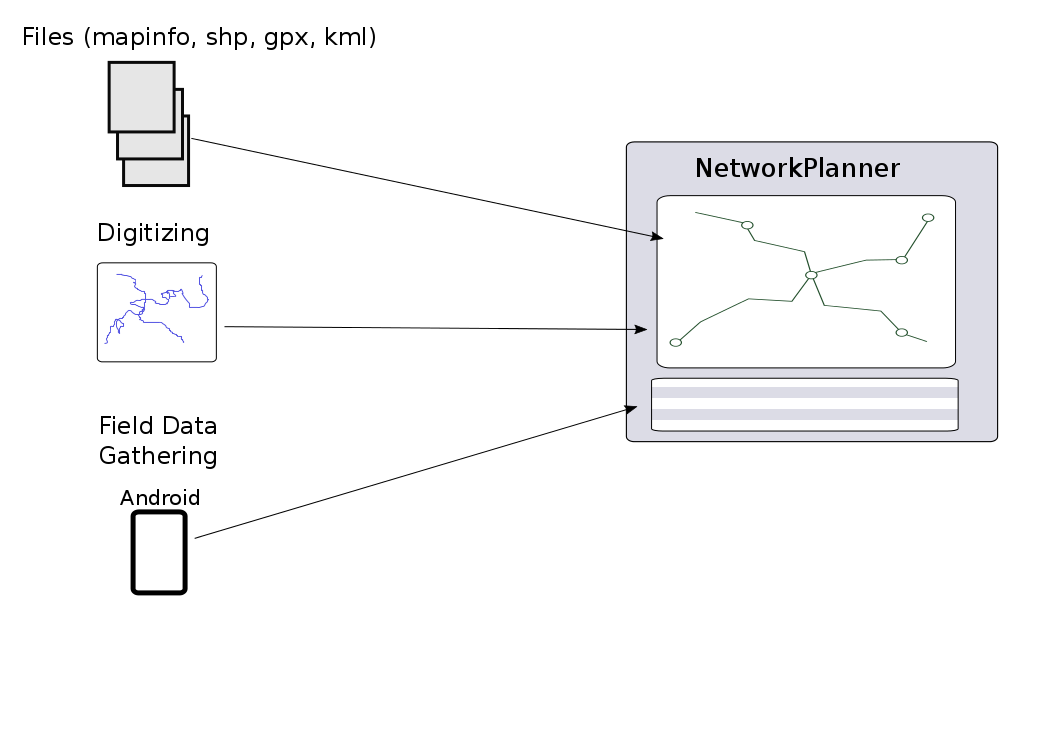
\includegraphics[width=4.5in,height=2.75in]{../diagrams/gridmaps-flow-original.png}
\end{frame}

\begin{frame}{Improved Workflow}
  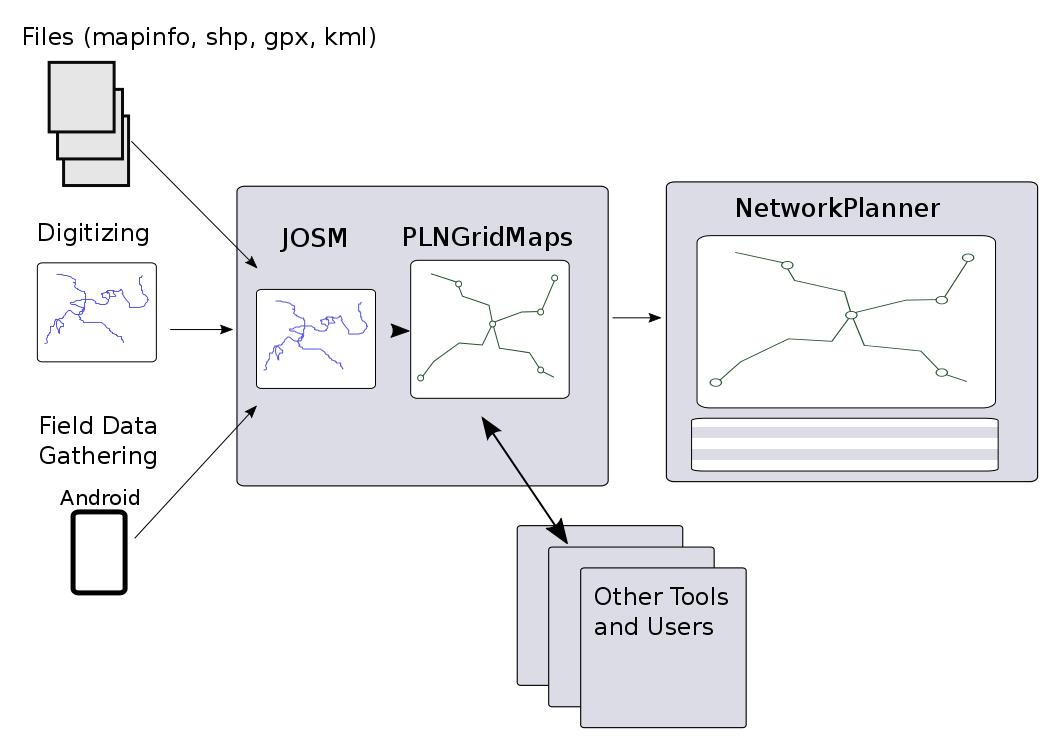
\includegraphics[width=4.5in,height=2.75in]{../diagrams/gridmaps-flow.png}
\end{frame}

\begin{frame}{JOSM}
  \begin{itemize}
  \item[] Quick demo of JOSM
  \item[] More details in separate doc
  \end{itemize}
\end{frame}

\begin{frame}{Export}

  \begin{itemize}
  \item[] Export KML of Sula from plngridmaps.com
  \end{itemize}
  
\end{frame}
\end{document}
